\chapter{Results}\label{chap:results}


Describe the experimental setup, the used datasets/parameters and the experimental results achieved

\section{Dataset}
In this implementation we used the following datasets: text8\footnote{matt mahoney} and ewik9\footnote{matt}, these are both repsectively the first 30 and 100MB of clean text from Wikipedia. We chosed the text8 dataset becaus it was already used in related work and is very small, giving us a fast computation time. We needed a second more larger dataset to confrim our results, and a dataset with specific vocabulary for us to be in roder to compute the analogy task (more on this in the results). The first document consists of 1702 documents of 10k word. No punctuation. 
 Therefore we needed to split the data set into sentences. We arbitrary chose a length of 20. Furthermore we applied subsampling (described in the next subsection)  too both of these datasets. For more information look at table stats.
\subsection{Subsampling}
Subsection is a technique introduced by Mikolov et al. in \cite{mikolov}. Certain words that appear very frequently in the dataset such as: "the, as, it, of". Do not give an intrinsic value to the words that appear in it's context. Therefore the idea of subsampling is to delete theim from the dataset. This will increase the computation time and should in theory increase the accuracy of the model. Another interesting fact of subsampling is that words that would not have appeard in the context of the word will now be it. 
Subsampling will be the first step of our preprocing. A word $w$ will be eliminated with the following probability:
\begin{equation}
P(w) = 1- \sqrt{{\frac{t}{f(w)}}}
\end{equation}
where $f(w)$ is the frecquency of w, and $t$ is a treshhold set empirecally. (Mikolov et al.)  recommends a value between $0$ and $1e-5$. We experimented with different values and $1e-4$, seemed the most suted. We did this analysis by looking at and random set of sentences and analyzed the best context pairs. 
\subsubsection{Min count}
We also applied a techniqued, called min count, we deleted every word thatt did not appeared more than 5 times in our dataset. We got this idea from gensim \cite{gensim}. Therer were a few words that had no meaning (aldk, ahdfo) VERIFY in our dataset. and a word that only appears one time will be very dependent on it's original setting which will influence the words tha appear in its context and will therefore not be a true value. Therefore we applied this technique. It should in theory, such as subsampling, improve both the accuracy and computation. 
\subsection{Specification of datasets}
\begin{itemize}
\item Text 8 original: \\
17 mio words\\
1702 docs of 10k words/ no sentences 
\item Applied subsampling:
8mio words.
1702 w of 5k words
\item Transformed to  250k sen of 20 words
\end{itemize}

\begin{table}[]
\begin{tabular}{|l|l|l|l|}
\hline
Dataset & Voc size & Numb of sentences (20) & Number of Sentences(length 20) with sampling \\ \hline
text8   & 250k     & 4000                   & 2000                                         \\ \hline
enwik9  & 750k     & 100000                 & 5000                                         \\ \hline
\end{tabular}
\caption{Specifications of the dataset}
\end{table}

\section{Word similarity}
Evaluating word embedding is not an easy task. We cannot split our data set into train and test set. Therefore we need to verify that our embedings are of quality with other techniques. We therefore define the principle of word similarity. We need to define a measure for our word embedings, if they are similar. We will use the cosine distance for this task. The cosine distance of vectors $v$ and $w$ is 1 minus the cosine of the angle between the two vectors. The cosine distance is 0 if two vectors are pointing in the same direction. It's 1 if they are 90 deg aparts from each other and 2 if they are pointing exactly in the opposited direction. It's calculated by taking the dot product of $v$ and $w$ and deviding it by the magnitude of $v$ and $w$ divided by each other. (equation x). We get
\begin{equation}
cos_dis(v,w) =1 - \frac{v \cdot w}{|v| |w|} 
\end{equation}
If we normalize the vectors then their the cosine angle becomes the dot product which allows us to compute the distance much faster using gpu's. 
\subsection{wordsim353}
To rate our word embedings we will need a dataset that gives us the similarity of words. This is exactly what wordsim353 is. It's 353 pairs of words rated by humans on their similarity. The score goes from 10 and 1, 10 being the most similar. We will rank our embedings on the pearson corelation coefficient between the cosine distance and the score attributed by humans. 
\begin{figure}[ht]
    \centering
			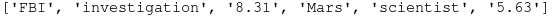
\includegraphics[scale=0.7]{images/wordsim353_example} 
    \caption{Example of pairs and their rating in wordsim353}
    \label{fig:efficient}
\end{figure}

\section{Configuration of the network}
The skip gram model, has a lot of possible options, that can be tuned. We configured one model and then only changed the learning rate. The explanation of the parameters will be structerd as follow: 
\texttt{Parameter} - Description and tuning -  \textit{Value}
\begin{itemize}
\item \texttt{Negative Samples} Here we have to find a trade off between, setting the parameter too high which will result in increased accuracy but a longer computation time. For smaller dataset a higher negative samples is often needed. We experimented early with 5, 10,15 - \textit{10}
\item \texttt{Context Window:} The bigger the window the more training examples the network will have, but if the window is to big the semantic meaning of the window will be erased. Mikolov et al. proposed a setting between 2-10. - \textit{5}
\item\texttt{ Dimension of the embedding}: Here the choice is less obvious, the higher the dimension the better the embedding should be.( cite paper dimension vectors talk about gensim ) but when tested on gensim 100 yielded better results than 300 - \textit{100}
\item \texttt{Batch size}: As described in section FORWARD, there is a trade off to find between accuracy and training time. We first used a batch size of 5000, but then decide after non conclusive results  that 2000 would be better - \textit{2000}
\item \texttt{Alpha}: learnng rate, this hyper parameter was tuned in every optimizer therefore only the range will be indicated - \textit{(1e-5,1)}
\end{itemize}

\section{Input Shuffling}
We used input shuffling as a technique to optimize the skip gram model. We will first describe input shuffling in a general way and then explain why we suppose that input shuffling could work well on the skip gram model. 
Let $X = {x_1...x_n}$ be our input data set. Input Shuffling describes the process of taking a random permutation of the dataset as an input at each epoch. 
The idea behind this technique, is the same as the use of mini batches. We want to present our optimizer with different loss surfaces, so that it's able to find the best optimum. But both combined can be a very powerful, there always lies a risk that a mini-batch isn't a good representative of the true gradient. This way, by shuffling the input, one would avoid this bias.
There are two reasons why we thnik that input shuffling is particulary well suited for the skip gram model. The first one has to do with the fact that when we read our words sequentially that words that only appear very early will not benefit from the context words being already updated from others. The second thing is that we used the special batch technique described in section x.  When using this technique and not using shuffling we will always have words that appear next to each other in a batch and will therefore updat similar words at the same time. We then loose some accuracy. But if instead we would use input shuffling then in one batch the words would likely not be similar and therefore overwriting will be less likely. 
One thing to consider is that when using input shuffling we cannot use a sliding window size. 

\section{Convergence time} 
To optimize convergence time we have to define convergence time first. Therefore we used the already available implementation gensim. we know from \cite{intel}. that a score of $0.66$ in the task of word similarity is the state of the art. We also know after testing Gensim ( more on this process in section discussion), that it takes 4 epochs to converge. Therefore we defined the following criteria for convergence: \\
$\rho - \rho_{prev} < 0.009 \vee or \rho = 0.66$ \\
where $\rho$ is the pearson coefficient with the wordsim353 task. 

\section{Results by optimizer}
\subsection{SGD}
The first think we had two manage was finding a correct learning rate for our model. We tried the learning rate from gensim first then expirmanted with different learning rates. As expected a bell curve shape resulted. the optimal setting that we found is $0.0075$. We converged in 11 epochs. 
We then added input shuffling to the equation. We see that for all the learning rates this helped to increase the convergenge time. Our models know converges in 7 epochs. An interesting point to notice is that we achieve this with a higher learning rate. 
\begin{figure}[h]
    \centering
			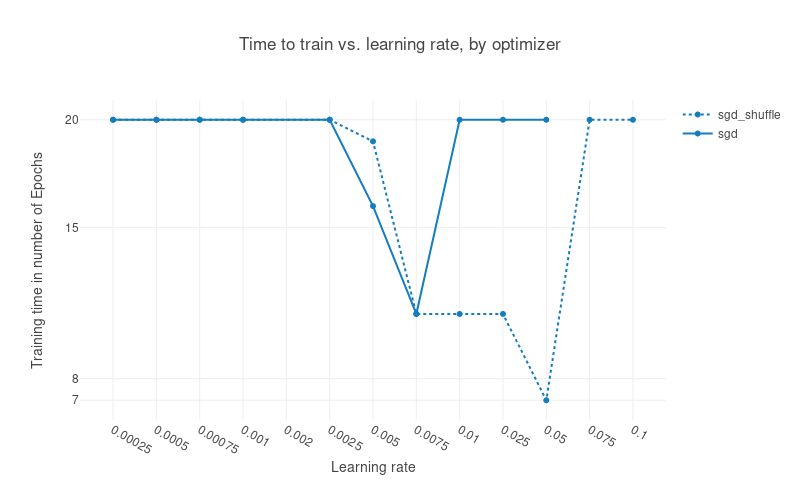
\includegraphics[scale=0.45]{images/results_sgd_shuffle} 
    \caption{Training time Stochastic Gradient Descent with input Shuffling}
    \label{fig:results_sgd}
\end{figure}
\subsection{Momentum and Nesterov}
Momentum and nesterov accelerated gradient both have an additional hyper parameter $\gamma$, that, as described in secction background, defines the importance of the previous gradient taking in the equation. We set $\gamma = 0.9|$ this is the typical value. Let's talk results: Momentum and NAG only slighltly respectively decrease or increasethe convergence time. NAG convergences in 12 epochs while momentum took 8 epochs. 
\begin{figure}[h]
\centering
\begin{minipage}{.5\textwidth}
  \centering
  	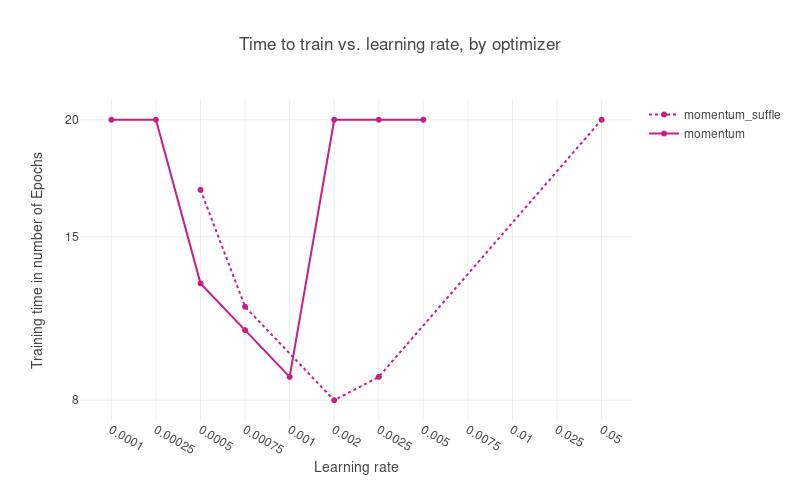
\includegraphics[scale=0.3]{images/results_mom_shuffle} 
    \caption{Training time  Momentum with input Shuffling}
    \label{fig:results_mom}
  \label{fig:test1}
\end{minipage}%
\begin{minipage}{.5\textwidth}
  \centering
	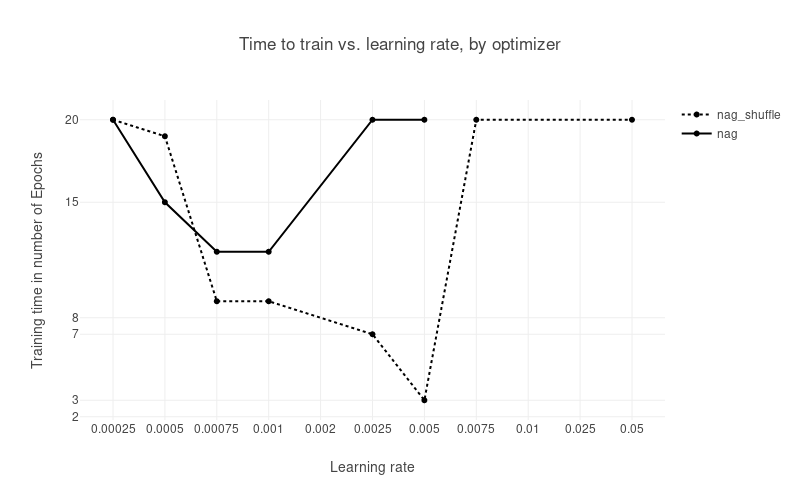
\includegraphics[scale=0.3]{images/results_nag_shuffle} 
    \caption{Training time  Nesterov with input Shuffling}
    \label{fig:results_mom}
\end{minipage}
\end{figure}
\subsection{Adagrad}
Adagrad is a very interesting tool for learning word embedding as they decrease the loearning rate for very frequent occuring features, and vice versa for low frequent words. Because words that appear very frequently often do not have a real semantic gain to their context words, it's good to have a low learning rate. this is also confirmed by the results adagrad converges in 4 epochs. When combined with shuffling adagrad only takes 3 epochs to converge. This shows the tendency of the skip gram model to converge faster with input shuffling.
\begin{figure}[h]
    \centering
			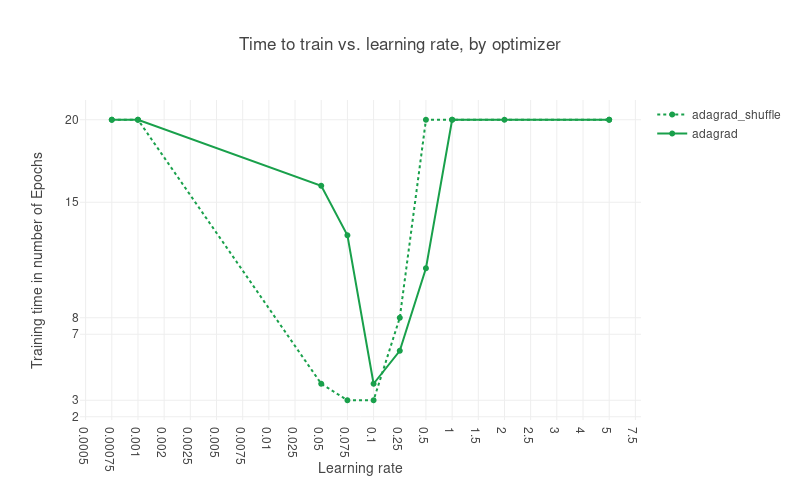
\includegraphics[scale=0.45]{images/results_adagrad_shuffle} 
    \caption{Training time Adagrad with input Shuffling}
    \label{fig:results_adagrad_shuffle}
\end{figure}
\subsection{Adadelta}
Adadelta was the Advanced optimizer that showed the most disapointing results. Because it didn't has any learning rate to tune, we only did 2 experiments, with and without input shuffling. the results where very much disapointing. Adadelta converged in 10 epochs with shuffling and 7 epochs without. Therefore barely beating sgd. This is interesting as Adadelta is an expansion of Adagrad, and is supposed, in theory to work better then the latter. 
\subsection{Adam}
Adam is the most advanced of all the optimizers used in our experiemnts. Did it therefore yield the best results? Indeed this was the case, as seen in figure 2, Adam converged in 3 epochs without shuflfling and 2 with. This are the best result that we got. 
\begin{figure}[h]
    \centering
			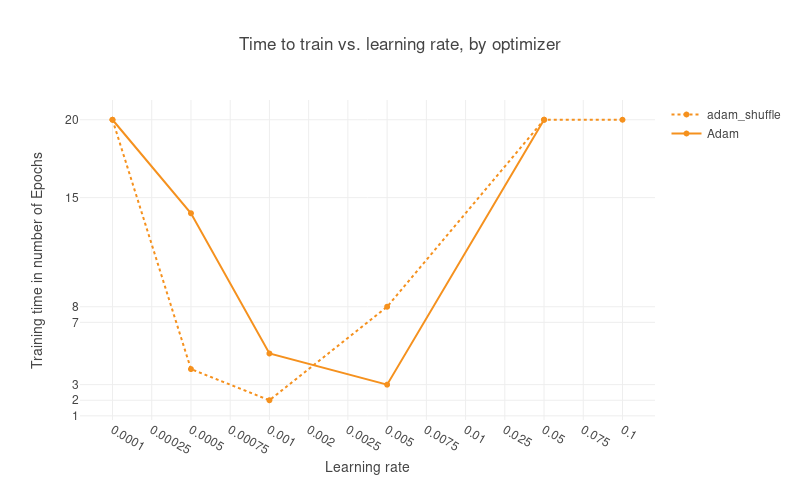
\includegraphics[scale=0.45]{images/results_adam_shuffle} 
    \caption{Training time Adam with input Shuffling}
    \label{fig:results_adam_shuffle}
\end{figure}